\section{استفاده از \lr{stack} برای ادغام}
\begin{frame}{ساختار \lr{\texttt{MergeState}}}
\begin{itemize}\itemr
\item[-]
ساختاری در کد‌هایی که مربوط به الگوریتم تیم‌سورت پیدا می‌شود به اسم \lr{\texttt{MergeState}}؛ این ساختار اطلاعات مورد نیاز برای توابع ادغام را داراست.

\item[-]
اطلاعات دیگری که در این ساختار نگهداری می‌شوند:
\begin{enumerate}\itemr
\item 
مقدار 
\lr{\texttt{min\_gallop}}

\item 
اندازه‌ی استک \lr{Run}ها:
\lr{\texttt{n}}

\item 
خود استک \lr{Run}ها:
\lr{\texttt{pending}}

\item 
آرایه‌ی موقت ادغام کردن:
\lr{\texttt{temparray}}

\item 
و سه تابع
\lr{\texttt{key\_compare}}،
\lr{\texttt{key\_richcompare}} و
\lr{\texttt{tuple\_elem\_compare}}
برای سناریو‌های مختلف مقایسه کردن بین عناصر آرایه.
\end{enumerate}
\vspace{-15pt}
\item[-]
کد این ساختار در اینجا\fn{1}{\url{https://github.com/python/cpython/blob/3.10/Objects/listobject.c\#L1185}}
قرار دارد.
\end{itemize}
\end{frame}

\begin{frame}{جلوگیری از اجرای بازگشتی}
\begin{itemize}\itemr
\item[-]
توابع بازگشتی وقتی که صدا زده می‌شوند، اطلاعات هر بار صدا زده شدن آنها، در
\lr{CPython}،
داخل آبجکتِ
\lr{frame}
آنها (\lr{frame}، آبجکتی است که اطلاعات و \lr{context} مورد نیاز برای یک \lr{code object} که حاوی \lr{byte code}‌های پایتون است را فراهم و ذخیره می‌کند) در یک \lr{stack} ذخیره می‌شوند،

\item[-]
اما آقای تیم پیترز این الگوریتم را که ماهیت بازگشتی مانندی دارد را غیر بازگشتی نوشته است و برای اینکار از یک \lr{stack} مخصوص خودش در سطح کد استفاده می‌کند.

\item[-]
هر بار که یک \lr{Run} پیدا می‌شود و اندازه‌ی آن به \lr{\texttt{minrun}} و یا بیشتر می‌رسد، اطلاعات آن روی \lr{stack} گذاشته می‌شود.

\item[-]
اگر بخواهیم ساده نگاه کنیم فرض می‌کنیم که خود \lr{Run} روی استک گذاشته می‌شود اما در واقع فقط آدرس شروع و اندازه‌ی آن روی استک ذخیره می‌شود تا از تکه تکه کردن آرایه و اشغال فضای بیشتر جلوگیری شود.
\end{itemize}
\end{frame}

\begin{frame}{استکِ \lr{\texttt{pending}}}
\begin{itemize}\itemr
\item[-]
این استک، نقاط شروع و طول هر \lr{Run} را در خودش ذخیره می‌کند.

\item[-]
این یعنی:

\lr{Run} عه
\lr{\texttt{i}}ام
از آدرس
\lr{\texttt{base[i]}}
شروع شده،
\lr{\texttt{len[i]}}
تا ادامه دارد و این عبارت همیشه درست است:
\begin{latin}
\begin{flushleft}
\texttt{pending[i].base + pending[i].len == pending[i+1].base}
\end{flushleft}
\end{latin}
\end{itemize}
\end{frame}

\begin{frame}{شروط استکِ \lr{\texttt{pending}}}
\begin{itemize}\itemr
\item[-]
برای اینکه اندازه‌ی \lr{Run}ها دقیقا و یا تقریبا با هم برابر بمانند تا الگوریتم‌های ادغام آنها را سریع‌تر ادغام کنند، هر بار که یک \lr{Run} جدیدی ساخته می‌شود اطلاعات آن روی استک گذاشته می‌شود، دو شرط برای \lr{Run}های روی استک چک می‌شوند.

\item[-]
اگر روی استک ما 
\lr{Run}های
\m{X}،
\m{Y} و
\m{Z}
وجود داشته باشند، این شروط باید حفظ شوند:
\begin{enumerate}\itemr
\item 
\m{|Z| > |Y| + |X|}
\item 
\m{|Y| > |X|}
\end{enumerate}
\vspace{-18pt}
\item[-]
شرط دوم بر این دلالت دارد که اندازه‌ی 
\lr{Run}ها
از بالا به پایین به صورت صعودی باشد و

\item[-]
شرط اول بر این دلالت دارد که وقتی از بالا به پایین می‌رویم طول \lr{Run}ها حداقل با سرعت دنباله‌ی فیبوناچی رشد کنند.
\item[-]
اگر هر کدام از این شروط نقض بشوند، 
\lr{Run} عه
\m{Y}
با \lr{Run} کوچک‌تر از بین 
\m{X}
یا 
\m{Z}
ادغام می‌شود و شروط دوباره چک می‌شوند و اگر برقرار بودند، الگوریتم به دنبال 
\lr{Run}
بعدی در آرایه جستجو می‌کند.
\end{itemize}
\end{frame}

\begin{frame}{شروط استکِ \lr{\texttt{pending}} (ادامه)}
\begin{itemize}\itemr
\item[-]
اگر
\m{|Z| \leq |Y| + |X|}
هر کدام از \m{X} یا \m{Z} که کوچک‌تر باشند، با \m{Y} ادغام می‌شوند (که الگوریتم \m{X} را ترجیح می‌دهد؛ بخاطر اینکه در کش تازگی دارد.)

\begin{figure}[H]
\begin{center}
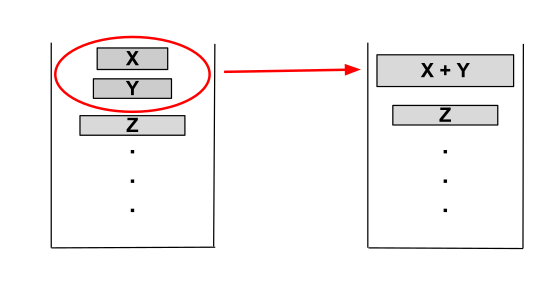
\includegraphics[width=0.5\textwidth, height=0.5\textheight]{docs/images/merge}
\end{center}
\end{figure}
\end{itemize}
\end{frame}

\begin{frame}{شروط استکِ \lr{\texttt{pending}} (ادامه)}
\begin{itemize}\itemr
\item[-]
برای مثال اگر این \lr{Run}ها را داشته باشیم:
\m{\left\langle Z:30 \quad Y:20 \quad X:10\right\rangle}،
\m{Y}
با
\m{X}
ادغام می‌شود:
\begin{lfl}
\m{\left\langle Z:30 \quad YX:30\right\rangle}
\end{lfl}

\item[-]
و یا اگر
\m{\left\langle Z:500 \quad Y:400 \quad X:1000\right\rangle}،
\m{Y}
با
\m{Z}
ادغام می‌شود:
\begin{lfl}
\m{\left\langle ZY:900 \quad C:1000\right\rangle}
\end{lfl}

که در هر دو مثال شرط دوم نقض می‌شود و الگوریتم تا زمانی که این دو شرط درست شوند، به ادغام کردن ادامه می‌دهد.

\item[-]
و در نهایت، تنها یک 
\lr{Run}
روی استک باقی می‌ماند که آرایه‌ی مرتب شده‌ی ماست.
\end{itemize}
\end{frame}


\begin{frame}{کدها}
\begin{itemize}\itemr
\item[-]
تابع 
\lr{\texttt{merge\_collapse()}}
\fn{1}{\url{https://github.com/python/cpython/blob/3.10/Objects/listobject.c\#L1955}}
مدیریت این شروط را به عهده دارد و انتخاب می‌کند که کدام \lr{Run}ها با هم ادغام شوند و این کار را با تابع 
\lr{\texttt{merge\_at()}}
انجام می‌دهد.

\item[-]
تابع
\lr{\texttt{merge\_at()}}
\fn{2}{\url{https://github.com/python/cpython/blob/3.10/Objects/listobject.c\#L1891}}
عمل ادغام تصمیمات مبنی بر اینکه ادغام باید با \lr{galloping} شود یا نشود را از نتایج توابع \lr{galloping} اتخاذ و عملیات ادغام با توجه به شرایط را با کمک توابع
\lr{\texttt{merge\_lo()}}
\fn{3}{\url{https://github.com/python/cpython/blob/3.10/Objects/listobject.c\#L1620}}
و
\lr{\texttt{merge\_hi()}}
\fn{4}{\url{https://github.com/python/cpython/blob/3.10/Objects/listobject.c\#L1751}}
انجام می‌دهد.
\end{itemize}
\end{frame}
